% Open Tasks
%
% --- General ---
% - Add keywords
% - Check universities' names
% - Correct typos and reformulate some paragraphs
% - ...
%
%
% --- Introduction ---
% - Citiations needed in parametric vs. nonparametric comparison part
% - Citiations needed on effect of environment
% - Section on how this work might be able to rule out certain alternative gravity models
% - Describe theoretical expectations (ellipticities of dm halo and luminous part, misalignments, effect of environment)
% - ...
%
%
% --- Data ---
% - More detailed description how the baryionic mass distribution was measured
% - More details needed on galaxies in the sample? I don't think so though
% - ...
%
%
% --- Method ---
% - Maybe more details on GLASS and how it works (cite Jonathan's upcoming paper)
% - Plot showing how well the shape informations is recovered when applied to fake data
% - Citation on why not monotonically decreasing radial density profiles are instable
% - Generally look through method part
% - ...
%
%
% --- Results ---
% - Interpretation of 
% - Interpretation of ellipticities plot (why it is relevant that dm halos are significantly rounder)
% - Interpretation of misalignment versus ellipticity plot ('forbidden region', alignment with semi-minor axis, very elliptical galaxies well aligned)




\documentclass[useAMS,usenatbib]{mn2e}
\usepackage{myaasmacros}
\usepackage{graphicx}
\usepackage{ulem}
\usepackage{amsmath}
\usepackage{multirow}


% Some definitions of things I always use here:
\newcommand\bcite[1]{\citeauthor{#1} \citeyear{#1}}


\title[Alignment of Light and Mass in Lensing Galaxies]{Alignment of Light and Mass in Lensing Galaxies}

\author[Bruderer]{Claudio Bruderer$^{1}$\thanks{E-mail: claudio.bruderer@phys.ethz.ch}, J. I. Read$^{2}$, P. Saha$^{3}$, J. Coles$^{4}$\\
$^{1}$Institute for Astronomy, Department of Physics, ETH Z\"urich, Wolfgang-Pauli-Strasse 27, CH-8093 Z\"urich, Switzerland\\
$^{2}$Department of Physics, University of Surrey, Guildford, GU2 7XH, UK\\
$^{3}$Institute for Theoretical Physics, University of Z\"urich, Winterthurerstrasse 190, 8057 Z\"urich, Switzerland\\
$^{4}$Department of Biology and Health, Versailles Saint-Quentin-en-Yvelines University, France
}

\begin{document}

\maketitle

\begin{abstract}
Understanding the structure and properties of galaxies today is essential to understand how galaxies formed. This poses a larger problem to us than one might imagine. Especially constraining the dark matter distribution in galaxy halos is not trivial. There are only a few methods to directly estimate this distribution. One of them is strong gravitational lensing, an effect caused by all of mass. This phenomenon allows constraining the gravitational potential of lens galaxies and thus the mass distribution. With knowledge of the light distribution it is possible to disentangle the dark matter and baryonic mass components and study their properties.
We use the newly-developped nonparametric framework \textit{GLASS} to model the mass distribution of a total of 15 strong gravitational lensing galaxies, most of which are early-type galaxies, for which we have information on the baryonic mass distribution. We are thus able to separate the mass components. By using a simple shape measure, namely the inverse of the moment of inertia tensor, we can analyze the shapes of the distributions. Analyzing the alignments between the semi-major axes of the distributions, we find that there can be significant misalignments and also cases of alignment between the semi-minor and semi-major axes. Mass thus need not follow light. Furthermore, the ellipticities of the dark matter distributions are always smaller than the baryonic mass distributions. Dark matter halos tend to be more spherical than the light distribution of the galaxy. We also consider the environment of the lenses. We find that lenses in denser environments tend to be more misaligned with either the semi-major or semi-minor axis. Additionally, the semi-major axis of lenses lying in groups or clusters of the dark matter halo might be oriented in direction of the centroid.
\end{abstract}

\begin{keywords}
asdf....
\end{keywords}


\section{Introduction}\label{sec:introduction}

\textbf{Context/Background/Motivation}
\begin{itemize}
\item Why interesting (lensing can constrain mass distribution (enclosed mass constraint independent from model with only few percent uncertainty e.g. Kochanek 1991?, Wambsganss \& Paczyński 1994?), insights into structure formation)
\item What is to be expected from theory (dm, alternative gravity)
\end{itemize}


\textbf{Anything done before?}
\begin{itemize}
\item Surely cite: \cite{1997ApJ...482..604K,1998ApJ...509..561K,2006ApJ...649..599K,2009ApJ...690..670T,2012ApJ...761..170G}
\end{itemize}


\textbf{New here}
\begin{itemize}
\item Statistics
\item Free-form modelling
\item group versus stellar misalignment with dm halo
\end{itemize}


Gravitational lensing is one of the few phenomena that allow probing the matter distribution directly. It makes no distinction between baryonic and dark matter, both components act on light rays in the same way. Gravitational lensing is therefore somewhat special as it allows to \textit{see} dark matter, if we are able to separate the two components. Therefore studying these effects allows us to probe dark matter and its properties. We are typically interested in measuring its distribution, how it clusters, its connection to structure formation, and of course its nature. With strong gravitational lensing galaxies we are effectively probing the matter distribution on relatively small scales. Thus, much insight could be gained in how galaxies form and how they are structured.

The main challenges are however first, estimating the baryonic mass distribution such that the two components can be disentangled (see e.g. \cite{leier11phd}), and second, modelling the lens, i.e. the mass distribution. This work focuses purely on the second aspect. There are in general two classes of methods to reconstruct gravitational lenses, parametric and nonparametric methods. A comparison of these two classes of methods can be found in \cite{2008ApJ...681..814C}. Parametric methods assume a distribution, which depends only on few parameters, such that the problem is well constrained and a best-fitting model can be found. They are computationally cheap, but on the other hand the assumption of a distribution might bias the result (CITATION NEEDED!). Nonparamatric (or free-form) methods assume a set of basis functions and find valid solutions in terms of linear superpositions of these functions. The problem is largely underconstrained. Due to the fact that there is no a priori reason to prefer specific mass models, given that they all satisfy certain prior conditions and reproduce the same gravitational lensing effects, over others, the best-fitting model is of little interest. Much more important is to explore many models and look at the properties of all the models in the ensemble. Typically high-dimensional parameter spaces, which describe all allowed models, need to be sampled in a uniform and uncorrelated way to generate a representative ensemble of solutions. The computational cost of these methods is usually much higher \citep{2008ApJ...679...17C,2012MNRAS.425.3077L}.

With these tools, we can start answering the long-standing question whether mass follows light. It is a well-known fact that for observations to match for example rotation curves of galaxies, the radial density profiles of baryonic mass and dark matter differ. The question is however whether baryonic mass and dark matter need to be aligned and the ellipticities need to agree. If this is not the case, then this needs to be explained by mechanism and effects that produce and sustain these different properties. Especially the environment of lenses might play a significant role (CITATION NEEDED!). It is furthermore unclear whether modified gravity theories could explain possible misalignments between mass and light.

There were already attempts to analyze the alignment of light and mass. \cite{1997ApJ...482..604K} use Singular Isothermal Spheres (SIS) with an external shear term and Singular Isothermal Ellipsoids (SIE) (e.g. \cite{1994A&A...284..285K}) without external shear to model the mass distribution. Applying this to a sample of 17 lenses, they find a strong correlation between light and dark matter distributions, if there is no strong external perturbation, with only a small scatter of less than $10^{\circ}$. They find however no correlation between the axis ratios of the distributions.

Later on, \cite{2006ApJ...649..599K} and \cite{2012ApJ...761..170G} analyzing lens samples of similar sizes and \cite{2009ApJ...690..670T} analyzing a lens sample containing even 70 galaxies also looked for misalignments. They all use SIEs to model the mass distributions. Only \cite{2012ApJ...761..170G} however include an external shear contribution in case more information is available. They neglect the external shear although \cite{1998ApJ...509..561K} find that SIEs with an independent external shear term fit the data better. They find reasonable alignments, the scatter is however larger than the one found in \cite{1997ApJ...482..604K}. \cite{2012ApJ...761..170G} find a rms scatter of $25^{\circ}$ for the whole sample. Even after dropping the almost spherical lenses, the rms scatter is still $18^{\circ}$. They attribute this to a significant external shear contribution. \cite{2009ApJ...690..670T} even find a significant correlation between the misalignment and the local and global environment. In general, lenses in overdense environments seem to be more likely to be misaligned. \cite{2009ApJ...690..670T} and \cite{2012ApJ...761..170G} also find a correlation with a large scatter between the ellipticities of the light and dark matter distributions.

Contrary to earlier approaches, we choose to use a non-parametric modelling technique. We use a pixel-based (see e.g. \cite{1997MNRAS.292..148S}) lens reconstruction framework called \textit{GLASS} \citep{2012MNRAS.425.3077L}. We apply this successfully on a sample of 15 strong gravitational lensing galaxies using stellar mass data of \cite{leier11phd}. Thus, we can disentangle dark and luminous matter and look at the shapes and alignments of these distributions. We can also look at the ellipticities of the reconstructed lenses and compare them to the ones of the stellar distribution. Furthermore, we discuss the environments of these lenses, as they might affect some properties of gravitational lenses in a significant way \citep{2006ApJ...641..169M,2011ApJ...726...84W}. We think that we have enough statistics to make claims about misalignments between the dark matter halo and the stellar mass distribution, and how the halo is oriented compared to the environment.

In Section \ref{sec:data} we present the lens sample and important properties of each lens. In Section \ref{sec:method} we present the reconstruction method we use and our shape measure. Section \ref{sec:results} consists of the results of this analysis. We show the relations we find between misalignment, ellipticities, and the environment.


\section{Data}\label{sec:data}
\begin{itemize}
\item SPS (Ignacio Ferreras, Dominik, etc. \citep{2011ApJ...740...97L})
\item Write why specifically these lenses were chosen, where they're from
\end{itemize}



\begin{table*}
 \begin{center}
  \begin{tabular}{l c c l || l c c l}
   Lens & $z_{L}$ & $z_{S}$ & Type & Lens & $z_{L}$ & $z_{S}$ & Type\\ \hline \hline
   Q0047 & 0.48 & 3.60 & Quad & HE1104 & 0.73 & 2.32 & Double\\
   Q0142 & 0.49 & 2.72 & Double & PG1115 & 0.31 & 1.72 & Quad\\
   MG0414 & 0.96 & 2.64 & Quad & B1152 & 0.44 & 1.02 & Double\\
   B0712 & 0.41 & 1.34 & Quad & B1422 & 0.34 & 3.62 & Quad\\
   RXJ0911 & 0.77 & 2.80 & Quad & MG2016 & 1.01 & 3.27 & Quad$^{1}$\\
   BRI0952 & 0.63 & 4.50 & Double & B2045 & 0.87 & 1.28 & Quad\\
   Q0957 & 0.36 & 1.41 & Double & HE2149 & 0.60 & 2.03 & Double\\
   LBQS1009 & 0.87 & 2.74 & Double & Q2237 & 0.04 & 1.69 & Quad\\
   B1030 & 0.60 & 1.54 & Double & & & & \\
%   SBS1520 & 0.72 & 1.86 & Double
%	B1600 & 0.41 & 1.59 & Double\\
  \end{tabular}
  \caption{List of all the lenses in the sample and their properties. Data is taken from \textit{CASTLES} and \cite{leier11phd}. The angles are measured north-through-east. \newline $^{1}$ Two images merge, thus only three images can be resolved.}
  \label{tab:overview}
 \end{center}
\end{table*}

\begin{table*}
 \begin{center}
  \begin{tabular}{l c c c c c c c}
   \multirow{2}{*}{Lens} & \multirow{2}{*}{Environment$^{a}$} & \multicolumn{2}{c}{Group/Cluster centroid$^{b}$} & & \multicolumn{2}{c}{Other galaxy} & \multirow{2}{*}{References$^{c}$}\\ \cline{3-4} \cline{6-7}
    & & $\Delta\alpha$ [''] & $\Delta\delta$ [''] & & $\Delta\alpha$ [''] & $\Delta\delta$ ['']\\ \hline \hline
   Q0047 & G(9) & $3.6\pm15.6$ & $43.2\pm28.8$ &   & ... & ... & 1\\
   MG0414 & 2 & ... & ... &   & $-0.4$ & $1.5$ & 2\\
   B0712 & 2 & ... & ... &   & $47$ & $-91$ & 3\\
   RXJ0911 & C & $-12.0$ & $-39.8$ &    & ... & ... & 4\\
   Q0957 & C & ... & ... &   & ... & ... & 5\\
   B1030 & 2 & ... & ... &   & $-9.8$ & $8.5$ & 6\\
   PG1115 & G(13) & $-10.8\pm21.0$ & $-3.6\pm15.6$ &   & ... & ... & 1\\
   B1422 & G(17) & $61.2\pm25.2$ & $-10.8\pm23.4$ &   & ... & ... & 1\\
%   SBS1520 & G(5) & ... & ... &   & ... & ... & 7\\
%   B1600 & G(17) & $-8.4^{d}$ & $-1.5^{d}$ &   & ... & ... & 8\\
   B1608 & G(8) & $-0.7$ & $8.0$ &   & ... & ... & 9\\
   MG2016 & C(69) & ... & ... &   & ... & ... & 10\\
   HE2149 & G & $-36.6$ & $14.2$ &   & ... & ... & 11\\
  \end{tabular}
  %$^{d}$ Only number-weighted estimates are available. \newline 
  \caption{List of lenses lying in a group or cluster environment, or that have a companion. \newline $^{a}$ G stands for group, C for cluster, and 2 means that the lens has a companion galaxy. If known, the number of member galaxies including the lens is given. \newline $^{b}$ If not stated differently, the centroid positions are luminosity-weighted estimates. \newline $^{c}$ References for the centroid estimates we used. \newline 1: \cite{2011ApJ...726...84W}; 2: \cite{1993AJ....105....1S}; 3: \cite{2002AJ....123..627F}; 4: \cite{2001ApJ...555....1M}; 5: \cite{1998ApJ...504..661C}; 6: \cite{2000ApJ...536..584L}; 7: \cite{2008ApJ...673..778A}; 8: \cite{2007AJ....134..668A}; 9: \cite{2003MNRAS.344..337T}; 10: \cite{2006ApJ...646...85W}; 11: \cite{2006ApJ...646...85W}}
  \label{tab:environment}
 \end{center}
\end{table*}

\begin{table*}
 \begin{center}
  \begin{tabular}{l c c c c}
   Lens & \multicolumn{3}{c}{Time delays [d]} & References\\ \hline \hline
   RXJ0911 & $\Delta t_{BA}=146\pm4$ & ... & ... & 1\\
   Q0957 & $\Delta t_{BA}=416.5\pm1.0^{a}$ & $\Delta t_{BA}=420.6\pm1.9^{b}$ & ... & 2\\
   HE1104 & $\Delta t_{BA}=162.2^{+6.3}_{-5.9}$ & ...  & ...  & 3\\
   PG1115 & $\Delta t_{BA}=12.0^{+2.4}_{-2.0}$ & $\Delta t_{DC}=4.4^{+3.2}_{-2.4}$ & ... & 4\\
%   SBS1520 & $\Delta t_{BA}=125.8\pm2.1$ & ... & ... & 5\\
%   B1600 & $\Delta t_{BA}=51\pm2$ & ... & ... & 6\\
   B1608 & $\Delta t_{BA}=31.5^{+2}_{-1}$ & $\Delta t_{CA}=36.0\pm1.5$ & $\Delta t_{DA}=77.0^{+2}_{-1}$ & 7\\
   HE2149 & $\Delta t_{BA}=103\pm12$ & ... & ... & 8\\
  \end{tabular}
  \caption{Lenses with measured time delays. $\Delta t_{BA}$ corresponds to the time delay between the images A and B with A leading. \newline $^{a}$ measured in the g-band \newline $^{b}$ measured in the r-band \newline 1: \cite{2002ApJ...572L..11H}; 2: \cite{2012A&A...540A.132S}; 3: \cite{2008ApJ...676...80M}; 4: \cite{2010MNRAS.406.2764T}; 5: \cite{2011A&A...536A..44E}; 6: \cite{2000ApJ...544..117B}; 7: \cite{2002ApJ...581..823F}; 8: \cite{2002A&A...383...71B}}
  \label{tab:timedelays}
 \end{center}
\end{table*}

The pixelated stellar mass maps we use, were reconstructed by \cite{leier11phd}. For each pixel the surface brightness was compared with stellar mass-to-light ratios, which were determined by stellar population synthesis models. This technique allows estimating the stellar mass in these pixels. Further details on this method can be found in \cite{leier11phd}, \cite{2005ApJ...623L...5F}, \cite{2008MNRAS.383..857F}.

Our sample originally consisted of 21 galaxies, identical to the one in \cite{leier11phd} and \cite{2011ApJ...740...97L}. As the lenses \textit{HS0818+1227}, \textit{SBS1520+530}, \textit{B1600+434}, \textit{B1608+656} proved too difficult to reconstruct, we dropped them from this analysis. The final sample consists thus of 17 galaxies. Most of these lenses are early-type galaxies except \textit{B1030+074}, \textit{B1152+200}, and \textit{Q2237+030}. All lenses can also be found in the gravitational lens database \textit{CASTLES}. Characteristics and references of each lens in the sample are listed below. Table \ref{tab:overview} contains all the redshifts and the type of the lenses, Table \ref{tab:environment} lenses with environment information, and Table \ref{tab:timedelays} lenses with measured time delays.

\textit{Q0047-2808} (hereafter \textit{Q0047}) is a luminous early-type galaxy \citep{1996MNRAS.278..139W}. \cite{2011ApJ...726...84W} find a group of 9 members all of which they spectroscopically confirm.

\textit{Q0142-100} (hereafter \textit{Q0142}) is a passively evolving early-type galaxy according to \citep{2000ApJ...536..584L,2007A&A...465...51E}.

\textit{MG0414+0534} (hereafter \textit{MG0414}) is a passively evolving early-type galaxy \citep{1999AJ....117.2034T}. \cite{1993AJ....105....1S} find a very close luminous satellite galaxy north-west of the lens. Due to the proximity of this satellite, we include it as a point mass in our analysis.

\textit{B0712+472} (hereafter \textit{B0712}) is an early-type galaxy \citep{1998AJ....115..377F}. Another galaxy, 102'' to the south-east seems to be at a similar redshift \citep{2002AJ....123..627F}. There is also a group of 10 galaxies at a lower redshift.

\textit{RXJ0911+0551} (hereafter \textit{RXJ0911}) is an almost circular early-type galaxy \citep{2012A&A...538A..99S}. It has measured time delays \citep{2002ApJ...572L..11H} and lies on the outskirts of a cluster \citep{2001ApJ...555....1M}. This cluster seems to be rather complex. Possibly it is not dynamically relaxed, although X-ray emission can be detected. Analysis of this emission yields a temperature of 2.3 keV. There is also a satellite galaxy to the north-west direction \citep{2000ApJ...544L..35K}.

\textit{BRI0952-0115} (hereafter \textit{BRI0952}) is an early-type galaxy \citep{2000ApJ...536..584L,2007A&A...465...51E}. \cite{2006ApJ...641..169M} find that the lens lies in a poor group of 5 members. However, a redshift of $z=0.41$ was used. According to \cite{2007A&A...465...51E}, the redshift is more likely to be $z=0.632$. They also find a system of 2 or 3 other galaxies at a slightly higher redshift of which the lens could be part of. The required external shear could be explained easily by a cosmic contribution \citep{2000ApJ...536..584L}. Therefore, we treat this lens as an isolated object.

\textit{Q0957+561} (hereafter \textit{Q0957}) is a cD galaxy lying close to the center of a cluster with a high sprial galaxy-fraction (e.g. \cite{1992MNRAS.254P..27G,1994A&A...291..411A,1998ApJ...504..661C}). Due to the large image separation, large physical scales are probed. As listed in Table 3 of \cite{2000ApJ...542...74K}, the position angles to the center of the cluster of earlier lens reconstructions range between 51.8 deg and 67.8 deg measured north-through-east. These results are consistent with the center of the X-ray emission from the cluster \citep{1998ApJ...504..661C}. The lens has a measured time delay (e.g. \cite{2012A&A...540A.132S}). They however also find a three-day lag between the g- and r-bands, and the estimates do not agree at the 2$\sigma$-level. They argue that this effect can be accounted for by the presence of a substructure and chromatic dispersion. We find that the results do not change significantly for either estimate and choose therefore the g-band measurement.

\textit{LBQS1009-0252} (hereafter \textit{LBQS1009}) is probably an early-type galaxy \citep{2000ApJ...536..584L}. \cite{2004A&A...428..741F} find no significant galaxy overdensity near the lens.

\textit{B1030+074} (hereafter \textit{B1030}) appears to have some substructure \citep{1998MNRAS.300..649X}. \cite{2000ApJ...536..584L} conclude that there are two distinct galaxies. The main one is a red, early-type galaxy. The other component seems to be fitted well by an exponential disk galaxy. They also conclude that no firm statements about the environment can be made. Although there is another galaxy nearby, it is too blue to be an early-type galaxy and thus they cannot estimate its shear contribution.

\textit{HE1104-1805} (hereafter \textit{HE1104}) is probably an early-type galaxy \citep{2000ApJ...536..584L,2000A&A...360..853C} and has measured time delays \citep{2008ApJ...676...80M}. \cite{2000ApJ...536..584L} also seem to find a group environment. \cite{2004A&A...428..741F} however conclude that the photometric redshift measurements of these galaxies indicate that they are at a higher redshift and rather associated with the source. Nonetheless, their lens models, parametric and free-form, all require strong external shear.

\textit{PG1115+080} (hereafter \textit{PG1115}) is an early-type galaxy \citep{2005ApJ...626...51Y}. It has measured time delays. We use recent estimates of the time delays by \cite{2010MNRAS.406.2764T} which differ significantly from traditional values by e.g. \cite{1997ApJ...489...21B}. \cite{2006ApJ...641..169M} and \cite{2011ApJ...726...84W} analyzed the environment of the lens thouroughly. It is part of a small group of 13 members. \cite{2004ApJ...610..686G} detect also X-ray emission from the corresponding group, which yields a temperature of 0.8 keV.

\textit{B1152+200} (hereafter \textit{B1152}) seems to have a color consistent with a late-type or an irregular galaxy \citep{2000A&A...357..115T}. Not much seems to be known about the environment of the lens.

\textit{B1422+231} (hereafter \textit{B1422}) is an early-type galaxy \citep{1996ApJ...462L..53I}. Although there are measured time delays by \cite{2001MNRAS.326.1403P}, they are probably not to be trusted too much as they deviate significantly from theoretical expectations in \cite{2003AJ....126...29R}. An accurate measurement of the time delays would require time delay measurements on the scale of hours. \cite{2006ApJ...641..169M} find a group environment with 16 spectroscopically confirmed member galaxies. Using newer data \cite{2011ApJ...726...84W} find an additional member. \cite{2004ApJ...610..686G} also detect X-ray emission from the corresponding group at a temperature of 1.0 keV.

%\textit{SBS1520+530} (hereafter \textit{SBS1520}) is an early-type galaxy, possibly with a disc \citep{2008ApJ...673..778A}. It has measured time delays \citep{2011A&A...536A..44E}. There is some uncertainty about the redshift of the galaxy. \cite{2002A&A...391..481B} find that their spectroscopic redshift estimate is consistent with $z=0.71$, which was measured first by \cite{1997A&A...318L..67C}. Both however also find a system at $z=0.82$, which could be the main lens. \cite{2002A&A...391..481B} however conclude that it is not associated with the lens. \cite{2008ApJ...673..778A} argue that a system they find at $z=0.76$ is more likely to be the lens, and the foreground system at $z=0.71$ is just a local perturber. Data seems however not conclusive. \cite{2008ApJ...673..778A} find and spectroscopically confirm a total of 3 groups along the line of sight. A poor group of 5 members is at $z=0.716$, another one with 13 members is at $z=0.758$, and a third group with 10 members is at a higher redshift $z=0.818$.

%\textit{B1600+434} (hereafter \textit{B1600}) is a nearly edge-on viewed late-type galaxy \citep{1997A&A...317L..39J}. The lens lies in a group with at least seven members, which all seem to be late-type galaxies \citep{2007AJ....134..668A}.

%\textit{B1608+656} (hereafter \textit{B1608}) consists of two merging galaxies. The main galaxy is an early-type galaxy which is disrupted by a smaller, probably late-type galaxy \citep{2003ApJ...584..100S}. The system has measured time delays \citep{2002ApJ...581..823F}. The environment and the mass distribution along the line of sight have been analyzed by \cite{2006ApJ...642...30F}. They find a group with 8 resp. 9 members if the merging galaxies are counted as 2. No significant X-ray emission was detected from the surrounding group \citep{2005ApJ...625..633D}. Along the line of sight seem to be four other groups.

\textit{MG2016+112} (hereafter \textit{MG2016}) is a giant elliptical galaxy \citep{1984Sci...223...46L,1986AJ.....91..991S}. It is the farthest lens we consider in this sample. It lies in a cluster which consists of 69 probable member galaxies \citep{2003MNRAS.344..337T}. The clusters shows a high density of galaxies close to the lens in a south-east direction.

\textit{B2045+265} (hereafter \textit{B2045}) is probably an elliptical galaxy \citep{2007MNRAS.378..109M}. \cite{1999AJ....117..658F} initially classified the galaxy as a late-type Sa galaxy, the velocity dispersion however seems too high. As the source redshift is rather low, a large lens mass is needed. \cite{2007MNRAS.378..109M} therefore conclude that it is more likely an elliptical galaxy. To the west of the lens, \cite{1999AJ....117..658F} find that a group at a similar redshift as the lens. \cite{2007MNRAS.378..109M} also find evidence for a dwarf satellite galaxy.

\textit{HE2149-2745} (hereafter \textit{HE2149}) is an early-type galaxy \citep{2007A&A...465...51E} and has a measured time delay \citep{2002A&A...383...71B}. There is some uncertainty in estimating the lens' redshift. Initial estimates by \cite{1996A&A...315L.405W} and \cite{2000ApJ...543..131K} found a probable redshift range of $\sim0.2-0.5$. By cross-correlating the lens spectrum with a template spectrum of an elliptical galaxy, \cite{2002A&A...383...71B} find that the redshift probably lies in the range $0.49\leq z \leq 0.60$, with the most likely redshift $z=0.495\pm0.01$. \cite{2007A&A...465...51E} however find that the redshift is more likely to be $z=0.603\pm0.001$. This would probably make the lens part of a poor group found by \cite{2006ApJ...641..169M} and \cite{2006ApJ...646...85W}. They also find two other groups at lower redshifts.

\textit{Q2237+030} (hereafter \textit{Q2237} or \textit{2237}) is a barred spiral \citep{1988AJ.....95.1331Y}. With only a redshift of $z=0.04$ it is the closest lens of the sample. Due to the low redshift, the probed physical scales are quite small. No further inquiries into the environment were made.

Further information about the sample can be found in \cite{leier11phd}, \cite{2011ApJ...740...97L}, and \cite{2012A&A...538A..99S}.


\section{Method}\label{sec:method}
\textbf{GLASS}
\begin{itemize}
\item Explain GLASS briefly and link to fake data tests
\end{itemize}

\subsection{Priors and assumptions}
\begin{itemize}
\item Explain what priors were chosen to model the lenses (Basically always pixrad 12, shear left free for quads, shear limited for doubles to 0.01, local gradient 50 degrees, smoothening prior 2, time delays if known. Exceptions are few. For some quads symmetry prior, for one double 0.01 was not possible therefore chose 0.1.)
\end{itemize}

\textbf{Shape measure}
\begin{itemize}
\item Explain shape measure
\item Link to tests on fake data
\item Include one plot of fake data test -> Jonathan
\item Illustrate everything with example lens PG1115.
\end{itemize}

In this work we use the new free-form lens modelling framework \textit{GLASS} \citep{2012MNRAS.425.3077L}. As its predecessor \textit{PixeLens} \citep{2004AJ....127.2604S}, it generates a pixelated mass map of a lens reproducing the image positions perfectly. Using pixels the arrival time surface for a source at position $\boldsymbol\theta_{S}$, taking the geometric and Shapiro contributions to the time delay into account, can be expressed in terms of the surface mass density rescaled by the critical density $\Sigma_{crit}$ of the n-th pixel $\kappa_{n}$ and the contribution to the gravitational potential of this pixel $\psi_{n}$ \citep{1997MNRAS.292..148S}
\begin{equation}\label{eq:arrival}
\tau(\boldsymbol\theta)=\frac{1}{2}|\boldsymbol\theta |^{2}-\boldsymbol\theta\cdot\boldsymbol\theta_{S}-\displaystyle\sum\limits_{n} \kappa_{n}\psi_{n}(\boldsymbol\theta).
\end{equation}

According to Fermat's principle, lensed images appear where the arrival time surface takes on extremal values $\nabla\tau(\boldsymbol\theta)=0$. Thus, the image positions fulfil
\begin{equation}
\boldsymbol\theta-\boldsymbol\theta_{S}-\displaystyle\sum\limits_{n} \kappa_{n}\alpha_{n}=0,
\end{equation}
where $\alpha_{n}$ is the contribution to the bending angle of the n-th pixel. For pixels, $\alpha_{n}$ and $\psi_{n}$ can be described by analytic formulae \citep{1997MNRAS.292..148S}. Reconstructing the lens, i.e. describing the surface mass density in every pixel, reduces thus to finding sets of coefficients $\left\{\kappa_{n}\right\}$ of these functions. As the number of pixels, which sets the resolution, is by far larger than the number of constraint equations in free-form modelling, this problem is highly underconstrained. The number of pixels is typically $\gtrsim 100$. We note that the equation is linear in $\kappa_{n}$. Also additional constraints on the lens such as individual time delays between images and their order and other priors we impose are linear. The volume of allowed solution is thus a high-dimensional polytope.

A fundamental difficulty in mass modelling is the non-uniqueness of solutions. They are not only not unique, every configuration which fulfils the equation is also equally probable. Therefore, this polytope needs to be sampled in a uniform way to analyze the full range of solutions. Due to the high dimensionality, sophisticated sampling methods of such volumes are required. \textit{GLASS} and \textit{PixeLens} differ in the method they use to sample such spaces. \cite{2008ApJ...679...17C} and \cite{2012MNRAS.425.3077L} show that \textit{PixeLens} does not produce uncorrelated random samples. They propose therefore a new sampling algorithm. They prove that generic high-dimensional polytopes indeed are sampled in a much more uniform way. Models in \textit{GLASS} are generated using a MCMC-method with a Metropolis-Hastings algorithm. A new step $x_{i+1}$ of the Markov chain is accepted with the probability
\begin{equation}
 \alpha = \mathrm{min}\left(1,\frac{P(x_{i+1})Q(x_{i},x_{i+1})}{P(x_{i})Q(x_{i+1},x_{i})}\right),
\end{equation}
where $P(x)$ is the probability distribution samples are drawn from and $Q(x_{i},x_{i+1})$ is the proposal density. As mentioned, all the valid mass configurations have the same probability, thus $P$ is a constant $\equiv1$. $Q$ has to be symmetric for Markov chains. It is usually taken to be a multivariate Gaussian $\mathcal{N}(x,\hat{\boldsymbol\Sigma})$, where $\hat{\boldsymbol\Sigma}$ is an estimate of the true covariance matrix $\boldsymbol\Sigma$. In principle it could be estimated by an adaptive chain during the random walk, but then the chain is no longer Markovian as it loses the reversibility property. Therefore, first an initial adaptive burn-in phase is run to get an good estimate $\hat{\boldsymbol\Sigma}$, before the real MCMC random walk. In this way, a large ensemble of models can be generated. The estimation of the covariance matrix is refined in \textit{GLASS} such that models are much less correlated. Further details and tests of the method can be found in \cite{2012MNRAS.425.3077L}.

\textbf{Priors and assumptions}
We use different priors and assumptions to eliminate unphysical mass reconstructions of the lens. First of all, the densities $\kappa_{n}$ need to be positive. As mass distributions with positive radial gradients are instable (CITATION NEEDED!), the density must always increase towards the center. Therefore, we require the local density gradient in every pixel except the central one to point towards the center within an angle of $50^{\circ}$. The radial density profile decreases monotonically, as required.

To avoid large fluctuations in the density, we choose to add a smoothing prior. The density in any pixel except the central one is at most twice the average density of its neighboring pixels. If there is reason to expect an invariant distribution under a rotation by $180^{\circ}$ (e.g. for doubles), we impose such a symmetry prior.

We also choose to include an additional external shear
\begin{equation}
  \gamma_{1}\left(\theta_{x}^{2}-\theta_{y}^{2}\right)+2\gamma_{2}\theta_{x}\theta_{y},
\end{equation}
which is added to (\ref{eq:arrival}) and the subsequent equations. We allow $\gamma_{1}$ and $\gamma_{2}$ to vary while fixing the maximum absolute value of the shear parameters. For doubles we fix the absolute value to be at most $10^{-2}$ (resp. $10^{-1}$ if no model could be generated for lower values ---> find out which galaxy and write this in more detail).

We further assume that the lens and image positions are perfectly known. As the range of possible models is much larger than the errors on these quantities, this assumption is justified \citep{2006ApJ...650L..17S}. We also fix a time order of the images. Furthermore, we choose a flat concordance cosmology with $\Omega_{m}=0.28$, $\Omega_{\Lambda}=0.72$, and $H_{0}^{-1}=13.7$.

\textbf{Shape measure}

To get a rough estimate of the shape of the surface mass distribution we use the inverse of the moment of inertia tensor of the mass map. Its eigenvectors and eigenvalues track the shape of the mass distribution. Thus, the shape is defined by two quantities; the ratio of the eigenvalues $\lambda_{1}/\lambda_{2}$, which describes the ellipticity, and the angle of the semi-major axis $\theta$. This seemingly crude measure was tested on fake data and found to be working well. (INPUT HERE FAKE DATA TEST)

Figure \ref{fig:1115rec} shows example plots of the reconstruction of the lens \textit{PG1115} illustrating this shape measure. In this lens system, there is a significant misalignment between the two mass distributions. 1$\sigma$- and 2$\sigma$-uncertainties on the angle estimates are shown. These errors are purely statistical, estimated by the ensemble of models. Figure \ref{fig:1115rec} also shows the arrival time surface and total, dark, and baryonic mass distributions.


\section{Results}\label{sec:results}
\begin{itemize}
\item Show some examples (stellar and dm contour plots, image of lens, arrival time surface, included mass)
\item Show money plots
\item Comment on a few lenses special lenses
\item Environmental effect?
\end{itemize}

\begin{figure*}
 \begin{center}%\hspace{-7mm}\hspace{0.8\textwidth}
  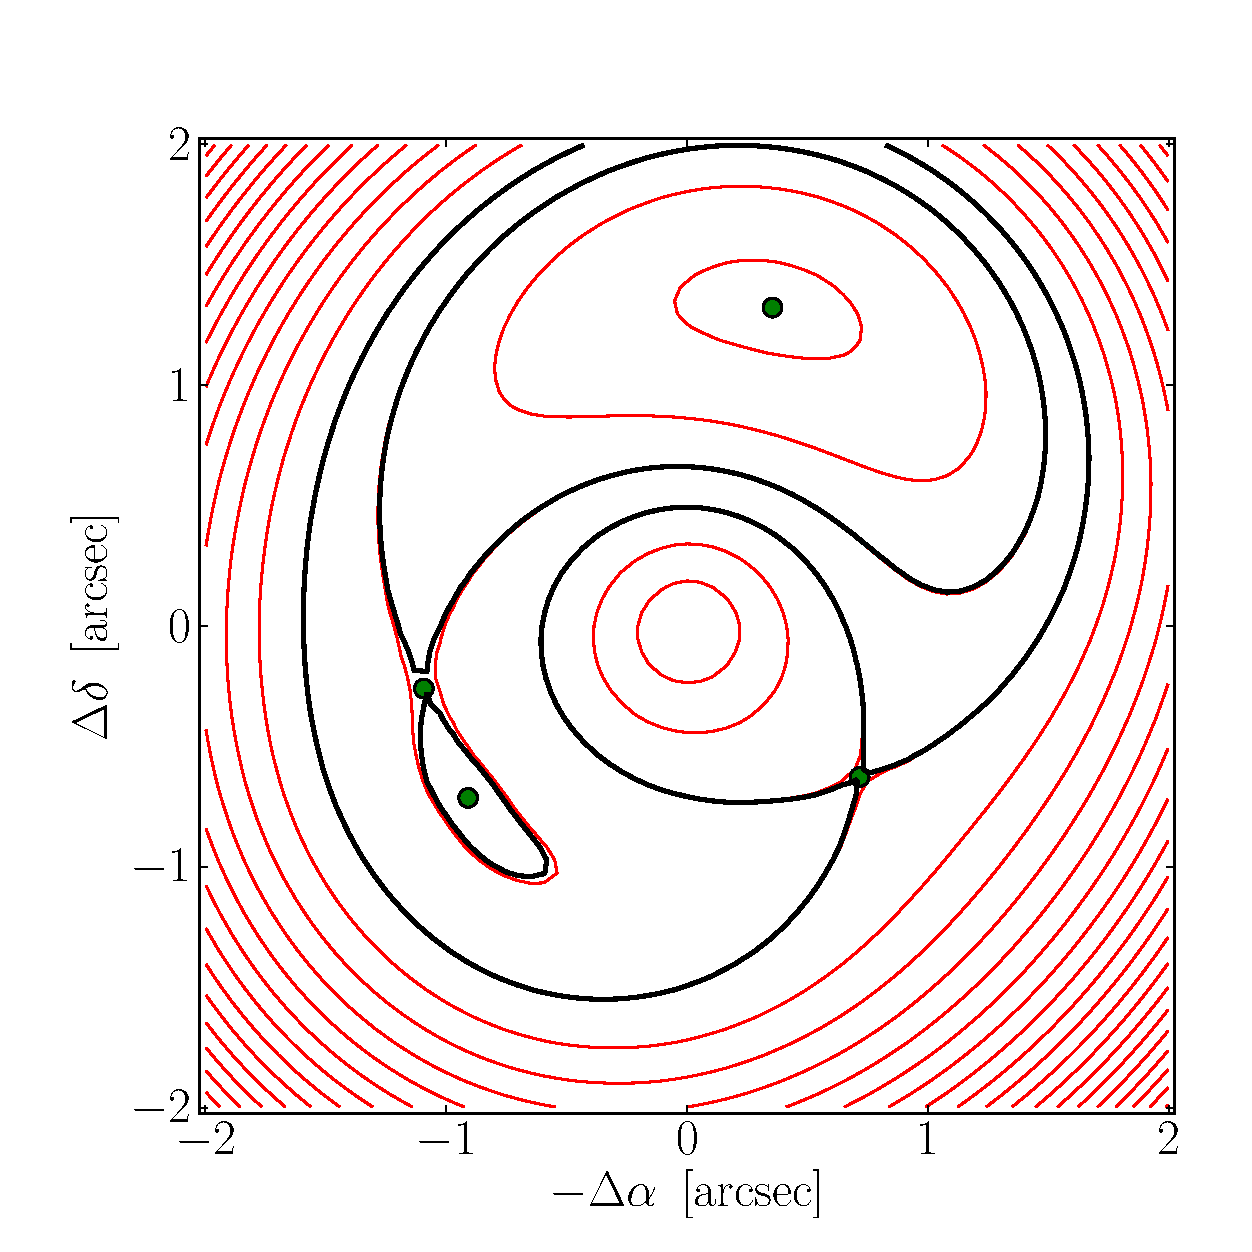
\includegraphics[height=0.32\textwidth]{Figures/1115_a.eps}
  \includegraphics[height=0.32\textwidth]{Figures/1115_b.eps}
  \includegraphics[height=0.32\textwidth]{Figures/1115_c.eps}\\
  \includegraphics[height=0.32\textwidth]{Figures/1115_d.eps}
  \includegraphics[height=0.32\textwidth]{Figures/1115_h.eps}\\
  \caption{Reconstruction of lens \textit{PG1115}. The plots show the mean model of the generated ensemble of models. The coordinate system is centered on the lens galaxy. (a) shows the arrival time surface. The green dots are the images, the red curves are isochrones, and the black curve are the lemniscate resp. the lima\c{c}on. (b) shows the total matter distribution. The red circle marks the circle of the outermost image. The green resp. cyan ellipses mark the shape of the dark matter resp. stellar distribution. This shape is measured as described in Section 3.3. In this case, the shape of the total matter distribution (black) is indistinguishable from the dark matter distribution. (c) shows the dark matter distribution. The black lines show the median semi-major resp. semi-minor axis with 1$\sigma$- and 2$\sigma$- uncertainties. The solid pink line points to the group centroid with $1\sigma$-uncertainties (dashed). (d) shows the luminous matter distribution.}
  \label{fig:1115rec}
 \end{center}
\end{figure*}

\begin{figure*}
 \begin{center}%\hspace{-7mm}\hspace{0.8\textwidth}
  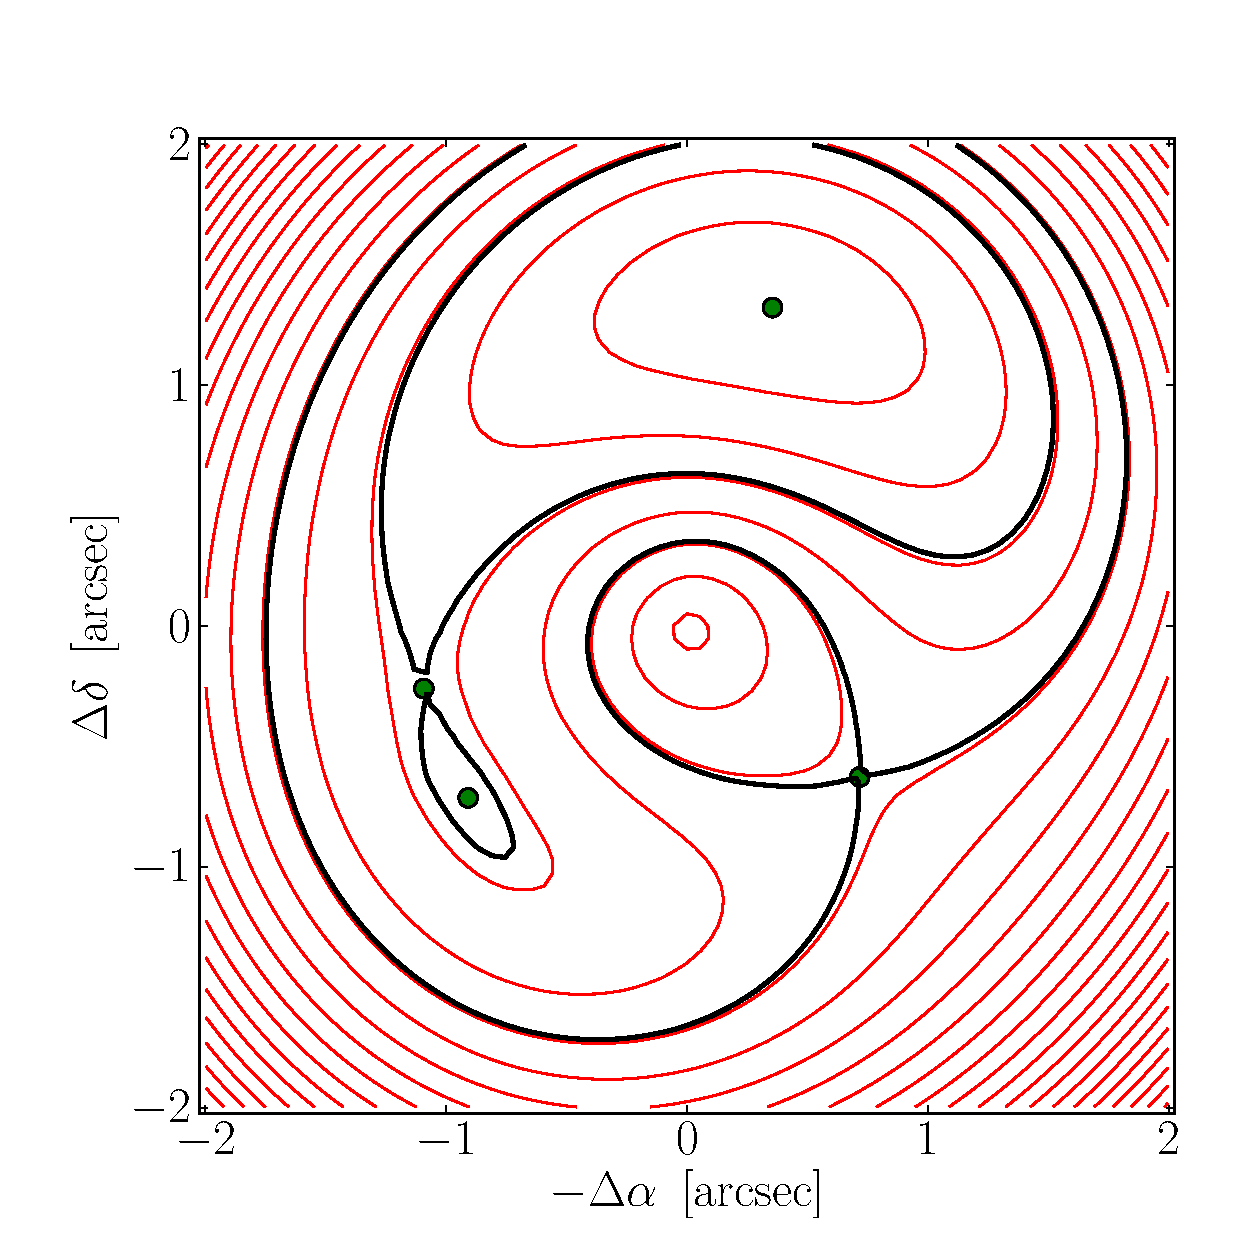
\includegraphics[height=0.32\textwidth]{Figures/1115_barkana_a.eps}
  \includegraphics[height=0.32\textwidth]{Figures/1115_barkana_b.eps}
  \includegraphics[height=0.32\textwidth]{Figures/1115_barkana_c.eps}\\
  \includegraphics[height=0.32\textwidth]{Figures/1115_barkana_d.eps}
  \includegraphics[height=0.32\textwidth]{Figures/1115_barkana_h.eps}\\
  \caption{Same as Figure \ref{fig:1115rec} but using time delay estimates from \cite{1997ApJ...489...21B}.}
  \label{fig:barkana}
 \end{center}
\end{figure*}

\begin{figure*}
 \begin{center}
 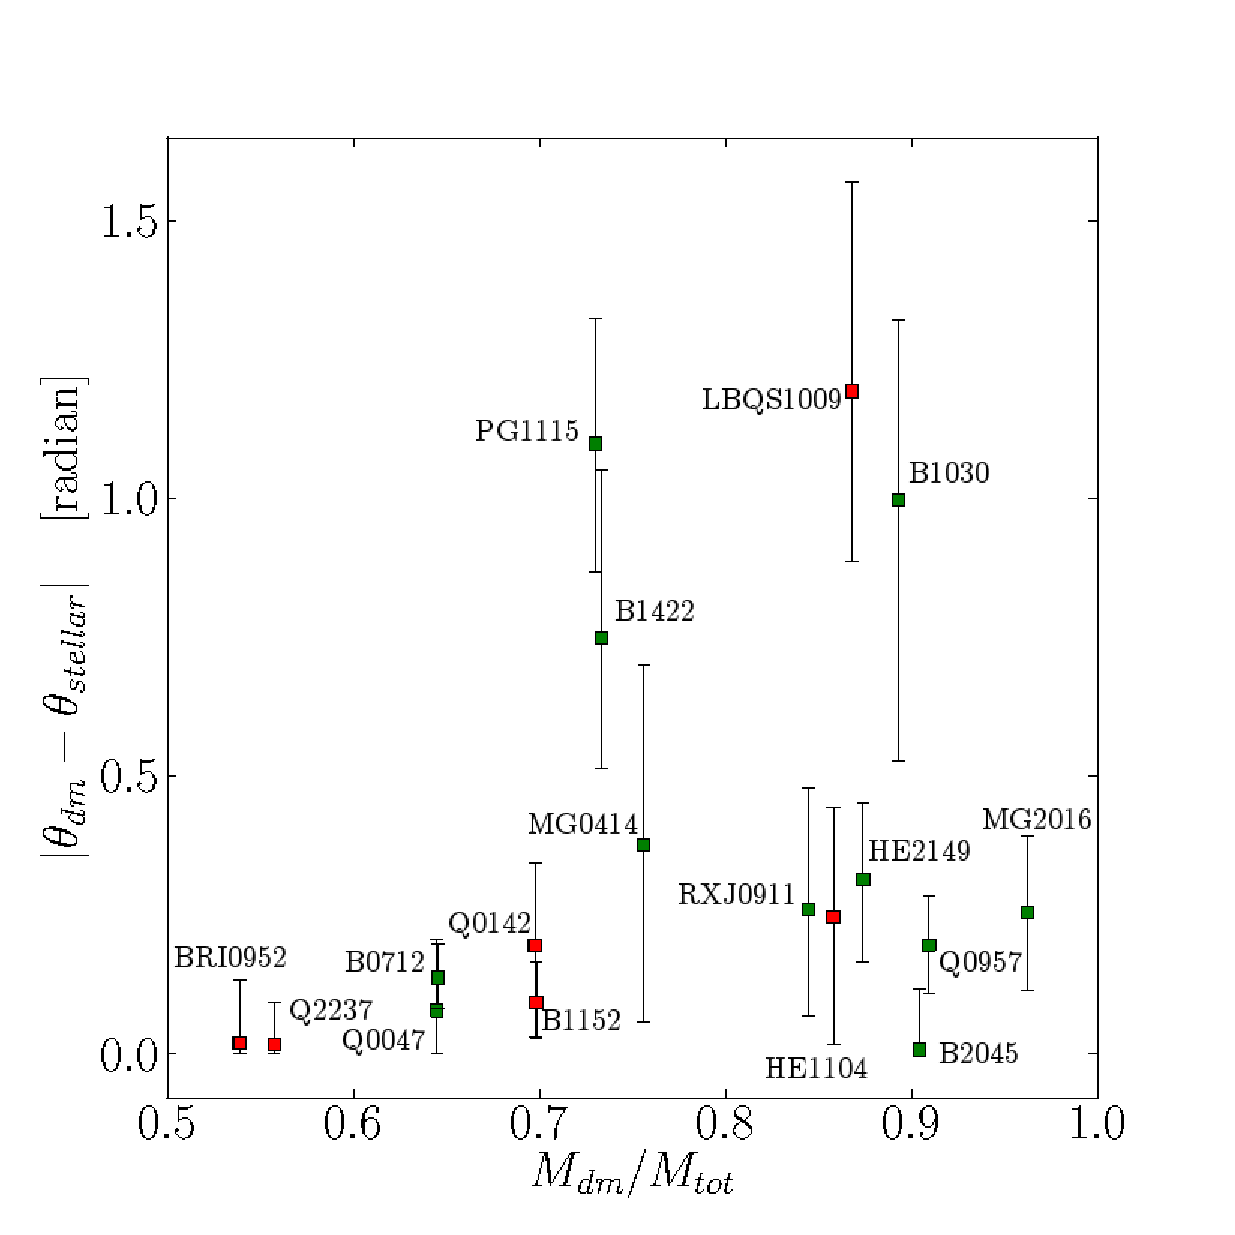
\includegraphics[height=0.49\textwidth]{Figures/b.eps}
 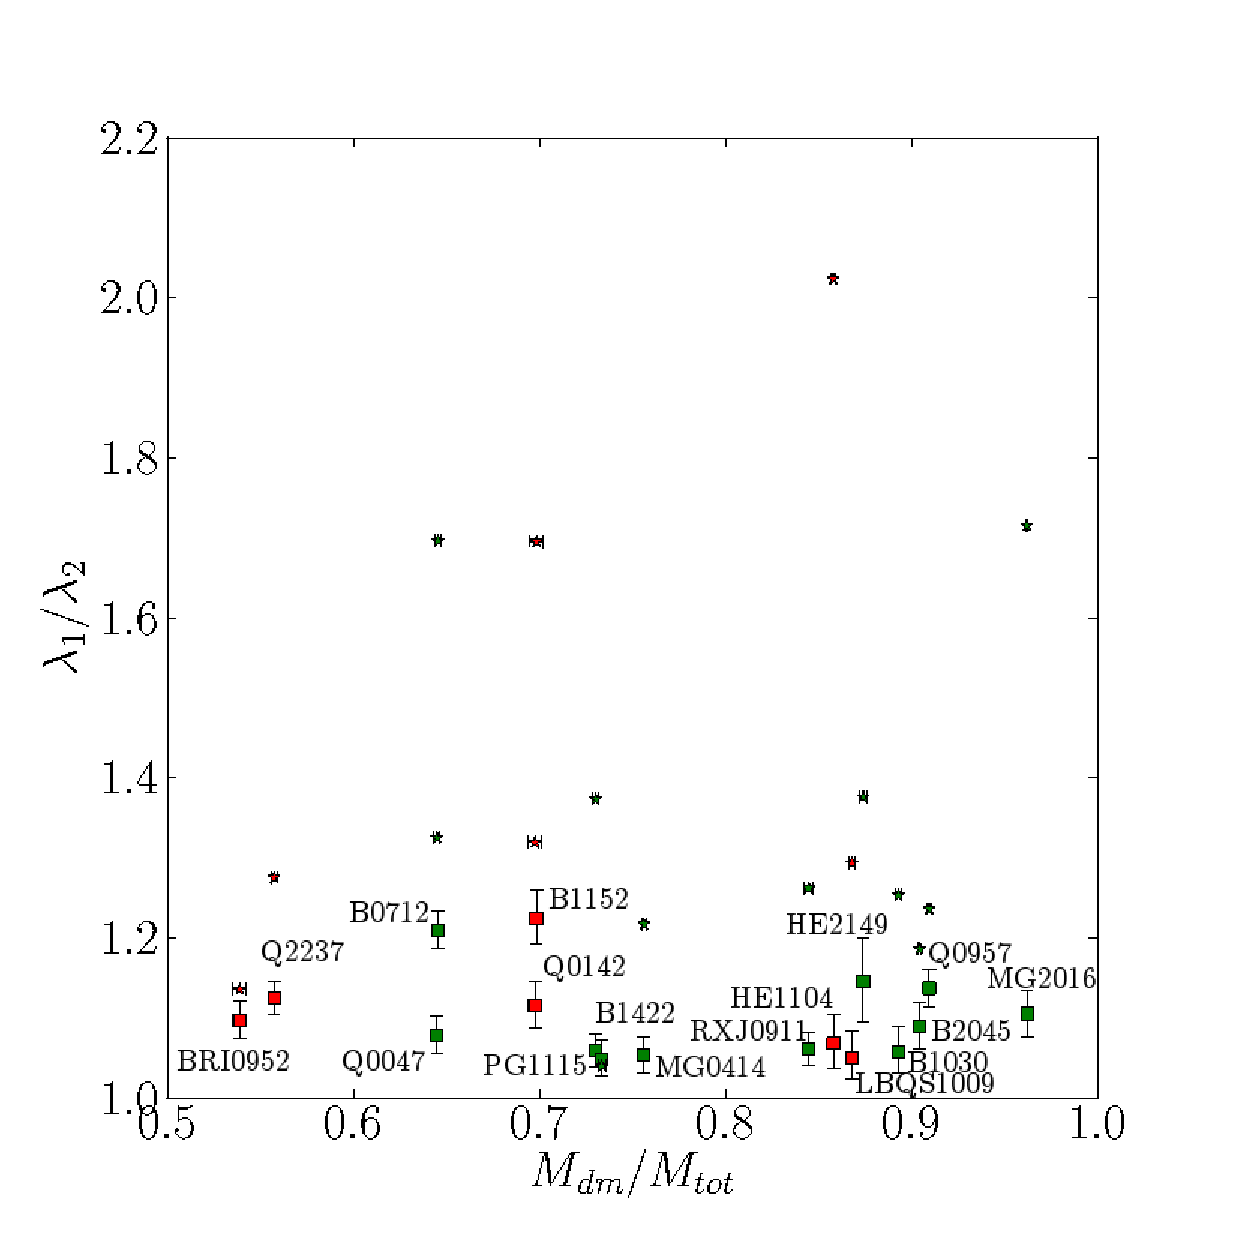
\includegraphics[height=0.49\textwidth]{Figures/d.eps}
 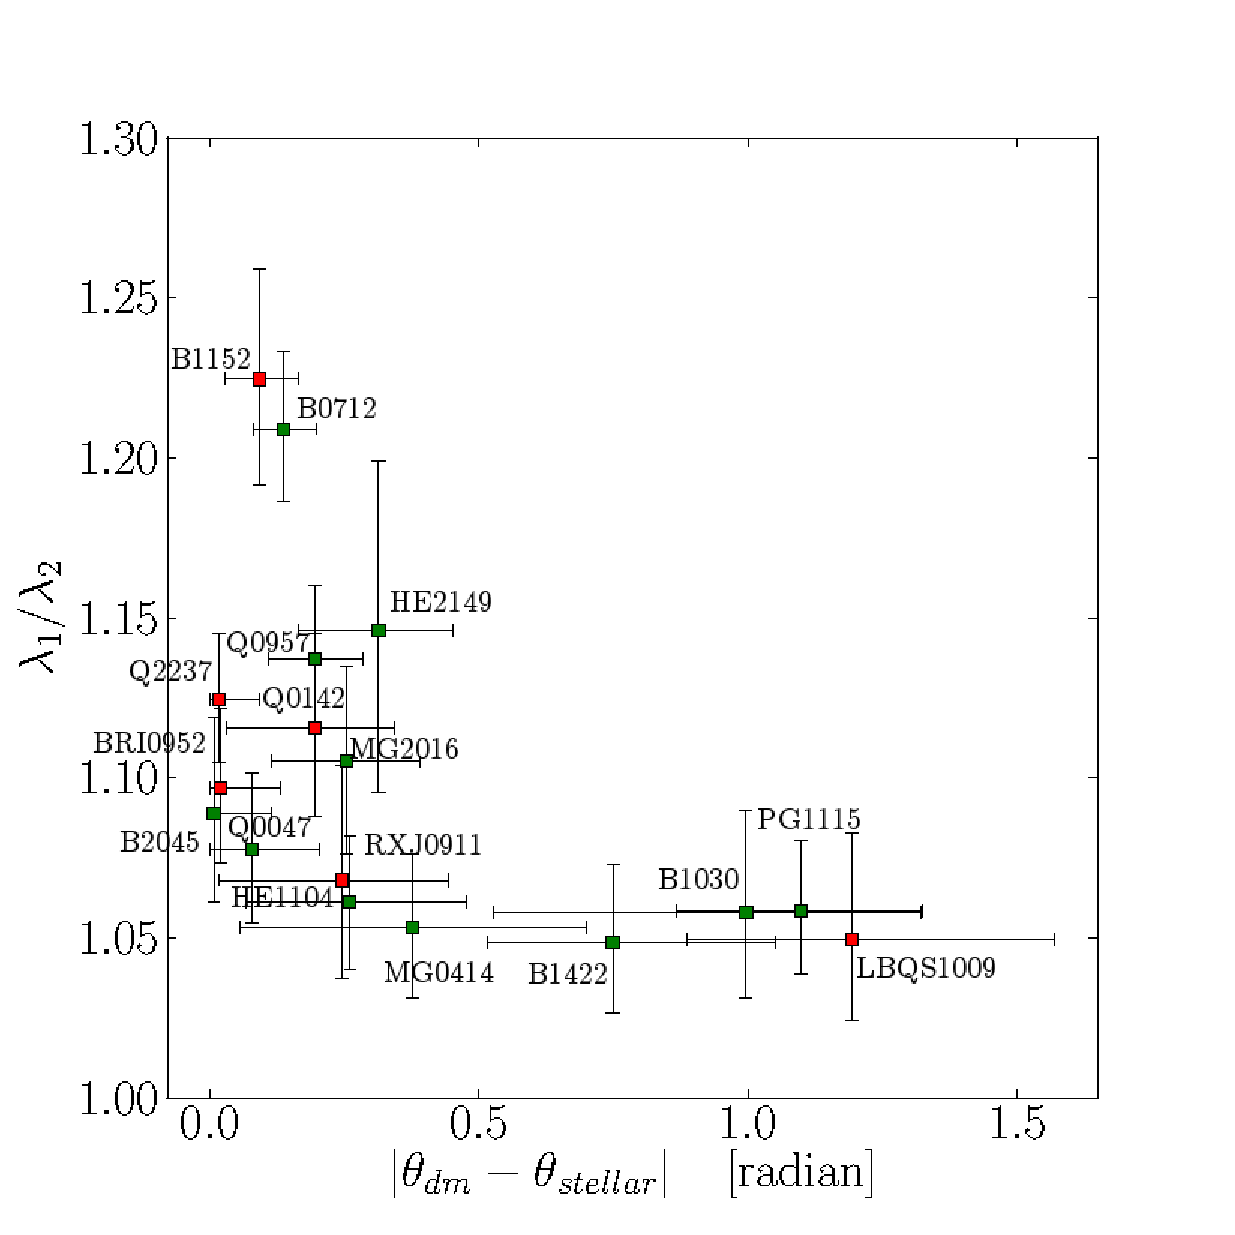
\includegraphics[height=0.49\textwidth]{Figures/e.eps}\\
 \caption{Plots of stellar and dark matter misalignments, ellipticities of the baryonic mass and dark matter distribution and a plot showing the ellipticity of the dark matter halo against the misalignment. Red symbols mark isolated objects or such without environment information, green symbols mark objects with at least one companion galaxy. In the second plot, stars denote the ellipticitie of the baryonic mass distribution, squares the ones of the dark matter halo.}
 \label{fig:moneyplots}
 \end{center}
\end{figure*}

\begin{figure}
 \begin{center}
 \includegraphics[height=\linewidth]{Figures/g.eps}
 \caption{Misalignment of the dark matter halo and the direction of the centroid of the environment.}
 \label{fig:environmentmisalign}
 \end{center}
\end{figure}


For every lens 10000 models were generated. This number allows for reasonable statistics, while not being computationally too expensive. In general an external shear of $\left|\gamma_{i}\right| \lesssim 10^{-1}$ is required to model quads. \textit{RXJ0911} and \textit{MG2016} however, need a significantly larger external shear of $\left|\gamma_{i}\right|\sim2\cdot10^{-1}$. This probably can be attributed to the cluster environments. As mentioned, the shear was limited to be $\left|\gamma_{i}\right| < 10^{-1}$ for doubles. The masses $M_{dm}$ and $M_{tot}=M_{dm}+M_{stellar}$ are always the masses included up to the radius of the outermost image.

%Our mass modelling shows that \textit{BRI0952} and \textit{Q2237} seem to have a rather large amount of mass in baryonic mass (e.g. Figure \ref{fig:moneyplots}). Also the two very massive, very dark matter dominated lenses \textit{Q0957} and \textit{MG2016} should be mentioned. \textit{Q0957} is a cD-galaxy and \textit{MG2016} a giant elliptical, so this result was to be expected.
%This can be explained for \textit{Q2237}. In \textit{Q2237} only the inner parts of the lens, where the baryonic mass dominates, are probed. 

Surprisingly, the shape measure we define yields are well-constrained results, as can be seen in Figures \ref{fig:1115rec} and \ref{fig:moneyplots}. The errors, which are purely statistical, on the ellipticities and the angles of the semi-major axis do not dominate the result. Lenses with almost spherical halos, i.e. $\lambda_{1}/\lambda_{2}\sim1$, should however be treated with caution.

As mentioned in Section \ref{sec:data}, there are different time delay estimates for \textit{PG1115}. We find that the results do not change much when using different estimates. As can be seen in Figure \ref{fig:1115rec} resp. Figure \ref{fig:barkana}, the dark matter distribution is a bit more spherical with the time delays from \cite{2010MNRAS.406.2764T} and the uncertainty on the angle of the semi-major axis grows. The misalignment we see is thus not affected by different time delays.

% The dark matter distribution in \textit{SBS1520} shows a very interesting behaviour. As can be seen in Figure \ref{fig:1520}, the dark matter seems to follow the baryonic mass distribution. Further out however, the dark matter distribution is rotated slightly. There is a significant misalignment between the dark matter distribution and the baryonic distribution. Without the central part, the misalignment would be even larger. This behaviour could be due to the potential disc \cite{2008ApJ...673..778A}, or caused by the many structures on the line of sight.














\textbf{Misalignments between stellar and dark matter distributions}
Figure \ref{fig:misalignment} shows the differences between the angles of the stellar and the dark matter semi-major axes versus the ratio of the included dark matter and total mass. For lenses with a significant stellar component inside the outermost image radius, the distributions seem to be rather aligned. It seems that if the luminous mass is comparable to the dark matter mass, then the distributions align. For a smaller stellar contribution this is not necessarily the case. The scatter increases and there can be significant misalignments, which can be seen especially clearly in the systems \textit{PG1115} (Figures \ref{fig:1115rec} or \ref{fig:tsvetkova})) and \textit{RXJ0911} (Figure \ref{fig:911}). While alignments between the distributions are preferred, they do not seem to be a necessary condition.

The environment might also play a role. Red are the systems, which are isolated or no group resp. cluster environment has been found, green the ones in such an environment. The misaligned systems are mainly the lenses with a known environment. Therefore, this misalignment could be caused by the external effects.


\textbf{Ellipticities of stellar and dark matter distributions}
The ellipticities of the distributions versus the mass ratio are shown in Figure \ref{fig:ellipticities}. We see, that every dark matter halo has a lower ellipticity $\lambda_{1}/\lambda_{2}$ and is thus closer to sphericity than the luminous galaxy. The systems \textit{HE1104} (Figure \ref{fig:1104}) and \textit{MG2016} (Figure \ref{fig:2016}) show especially large differences. It is not clear what could cause these

Figure \ref{fig:misalignmentellipticities} shows the misalignment versus the ellipticity of the dark matter halo. There seem to be five different regions. Almost spherical halos with good alignment of the semi-major axes, almost spherical halos with good alignment of semi-major and semi-minor axes (maximum misalignment between the semi-major axes), more elliptical, alligned halos, a seemingly 'forbidden' region for misalignments in between, and the upper right triangle, i.e. larger ellipticities and misalignments, which also seems forbidden. Understanding Figure \ref{fig:misalignmentellipticities} is certainly not trivial. Alignment with the semi-minor axis might be a stable configuration for almost spherical halos, while slightly smaller misalignments are unstable. There also seem to be some outliers as \textit{PG1115}, \textit{SBS1520}, and \textit{HE2149}.


\textbf{Misalignments between the dark matter distributions and environment}
Figure \ref{fig:environment} shows the misalignment between the direction to the group or cluster centroid resp. the companion galaxy with the dark matter halo. Although the error bars are huge, we immediately see that three lenses are basically aligned with the environment. The four other systems show slight misalignment. Having a closer look at these lenses shows however that at least two of them might in fact be aligned. For \textit{RXJ0911} and \textit{HE2149} there are no errors on the estimates of the centroid. Otherwise they would probably agree very well. \textit{Q0047} does not seem to be aligned with the direction of the group centroid. This could be due to the fact that the lens itself is quite far away from the centroid. The halo of \textit{B1030} is almost spherical, so the apparent misalignment could maybe be explained. It is also the only lens with only one companion galaxy. It is possible that in this case the effect of the environment is not strong enough. We however certainly lack data to make any claims for the systems with just one companion galaxy. Then, there is also \textit{MG2016}, which is not shown here, as the centroid was not measured in this cluster. There is however a high galaxy density towards the south-east, where also the cluster centroid probably lies. Judging from Figure \ref{fig:2016}, the halo seems to be aligned with the cluster centroid.

We conclude that lenses in groups or cluster are maybe aligned with the centroid. However, as we lack the statistics and as the errors on the centroid positions are huge, this claim might be disproved. It is not possible at this point to make a similar statement for lenses with just one companion galaxy.


\section{Conclusion}\label{sec:conclusion}
\begin{itemize}
\item Recapitulate what were the main results
\item Answer whether this method is promising
\item What is needed to understand such misalignments better (-> Surely need to understand environment effects better, ...)
\end{itemize}

We used a nonparametric modelling method to reconstruct a total of 15 lenses. Using previously measured light maps, then converted to luminous mass maps \cite{leier11phd}, we were able to isolate the dark matter distribution. We used the eigenvalues and eigenvectors of the inverse of the moment of inertia tensor to characterize the shape of the light and mass distributions. This allowed us to analyze the alignment between these distributions and the relation between the ellipticities. Furthermore, we included environment information, which we related the to the misalignment.

Our results can be summarized in the following way. If lenses lie in dense environments, mass and light need not be aligned. This might also be the case for lenses without known environments. We found more scatter than previous analyses by \cite{1997ApJ...482..604K}, \cite{2006ApJ...649..599K}, \cite{2009ApJ...690..670T}, and \cite{2012ApJ...761..170G} which all used SIEs mostly neglecting external shear to model the lenses. We also found that the semi-major and semi-minor axes of the distributions can be aligned, if the dark matter halos are close to sphericity. Up to our knowledge, this result was not obtained in other analyses.

We found that dark matter halos are rounder than the luminous galaxies, i.e. they have a lower eigenvalue ratio $\lambda_{1}/\lambda_{2}$. Previous analyses found a correlation between the ellipticities \citep{2009ApJ...690..670T,2012ApJ...761..170G}, which we do not see. They also found a couple of cases, where the stellar distribution is more spherical than the dark matter halo. We claim that certain combinations of ellipticity of the dark matter halo and misalignment between light and mass seem to be forbidden. However, more lens systems are needed to support this claim.

We suspect that the dark matter halo might be aligned with the centroid of the group or cluster it lies in. Due to the large uncertainties in the centroid positions however, such alignments might as well be coincidences.

We want to stress again that the systems \textit{SBS1520} and \textit{PG1115}, which both show some misalignment and have time delay measurements, seem interesting enough to investigate further. In \textit{SBS1520} we found that the outer parts of the dark matter distribution is rotated respective to the central, which displays an interesting feature possibly due a disc. It is on the other hand a very complicated system with a lot of structures along the line of sight. \textit{PG1115} is easy to model, but still shows a clear misalignment. Thus, it could serve as a test for other methods that try to reproduce these misalignments.


\section{Acknowledgements}\label{sec:acknowledgements}
Acknowledge Dominik Leier...

JIR would like to acknowledge support from SNF grant PP00P2\_128540/1.

\bibliographystyle{mn2e}
\bibliography{paper}

%\clearpage
\appendix
\section{Reconstructed Lenses}\label{sec:reconstructions}

\begin{table*}
 \begin{center}
  \begin{tabular}{l c c c c l l}
   Lens & A & B & C & D & Symmetry & Point Masses\\ \hline \hline
   Q0047 & 1.083 & 1.083 & 1.083 & 1.083 & Yes & $-\Delta\alpha = 2.301$ , $-\Delta\delta = 2.301$ , Mass range: $10^{7}-10^{9} \mathrm{M_{Sun}}$\\
   Q0142 & & & & & & \\
   MG0414 & & & & & & \\
   B0712 & & & & & & \\
   RXJ0911 & & & & & & \\
   BRI0952 & & & & & & \\
   Q0957 & & & & & & \\
   LBQS1009 & & & & & & \\
   B1030 & & & & & & \\
   HE1104 & & & & & & \\
   PG1115 & & & & & \\
   B1152 & & & & & \\
   B1422 & & & & & \\
   B1608 & & & & & \\
   MG2016 & & & & & \\
   B2045 & & & & & \\
   HE2149 & & & & & \\
   Q2237 & & & & & \\
  \end{tabular}
  \caption{...}
  \label{tab:lensparameters}
 \end{center}
\end{table*}

\end{document}
